\section{Results}
\label{sec:results}

All numbers below are produced by \texttt{experiments/make\_figures.py} from the
code described in Sec.~\ref{sec:numerics}; the planetary elements are
approximate J2000 mean elements (Sec.~\ref{sec:discussion}), so the results
test the expansion and its truncation machinery against exact two-body motion
and against an N-body integration, not against an ephemeris.

\subsection{Coefficient decay}
\label{sec:res-decay}

Figure~\ref{fig:decay} shows $|c_k|$ and $|c_{-k}|$ of the Kepler Fourier
series (Prop.~\ref{prop:series}) for $e\in\{0.0934,0.25,0.6,0.89\}$. The
coefficients decay geometrically at the Kapteyn rate
$\rho(e)^k$, $\rho=e\,e^{s}/(1+s)$, $s=\sqrt{1-e^2}$, with
$\rho=0.127$, $0.334$, $0.742$ and $0.964$ respectively. Retrograde terms
are smaller than prograde terms by roughly $(e/(1+s))^2$ at small $k$.
The formulas themselves reproduce the exact Kepler solution
to $10^{-14}$ (in units of $a$) at $e=0.5$ with $60$ harmonics.

\begin{figure}[H]
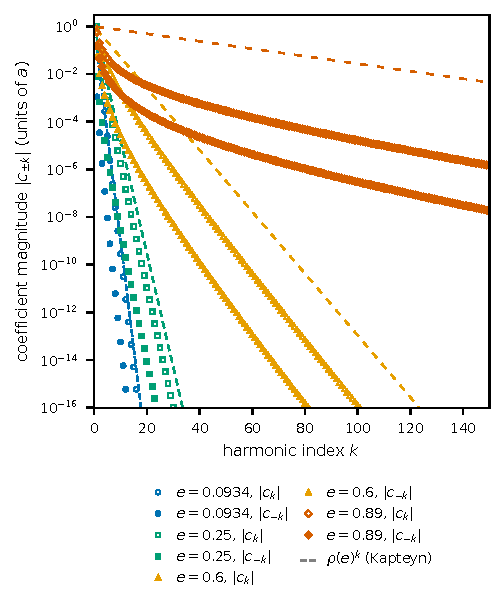
\includegraphics[width=\columnwidth]{fig_coeff_decay.pdf}
\caption{Magnitude of the Kepler-orbit Fourier coefficients $|c_k|$ (open
markers, $k>0$, prograde) and $|c_{-k}|$ (filled markers, retrograde; marker
shape distinguishes $e$) in units of $a$, for $e\in\{0.0934,0.25,0.6,0.89\}$
(Mars, and three illustrative values; $e=0.89$ is Phaethon). Dashed lines:
the Kapteyn rate $\rho(e)^k$.}
\label{fig:decay}
\end{figure}

\subsection{Geocentric convergence}
\label{sec:res-conv}

Figure~\ref{fig:conv} shows the maximum geocentric error over a $50$-yr window
(daily samples) of the truncated chain with $N_{\rm body}=N_\oplus=N$,
against exact Kepler motion, together with the rigorous tail bound
$\varepsilon_N(\text{body})+\varepsilon_N(\oplus)$. The bound is respected
everywhere and the error saturates at the double-precision floor,
$\sim2\times10^{-13}$~AU. The smallest sampled $N$ for which the error is below
$10^{-6}$~AU is $6$ for Mars, $6$ for Ceres and $240$ for Phaethon, and below
$10^{-9}$~AU it is $10$, $10$ and $450$. The cost is therefore
$2N=12$ to $20$ rotating circles plus a static offset per orbit ($24$ to $40$ rotating circles plus one combined offset in the geocentric chain) for planet-like eccentricities and of order a thousand for
$e=0.89$, consistent with the steep growth of the certified order
$N_{\rm cert}\propto(1-e)^{-3/2}$ (not the asymptotic behaviour of the actual
minimal order; Table~\ref{tab:nearpar}). For the single-body series
the observed $N$ for a sup error below $10^{-12}a$ is $12$ for Mars and
$575$ for $e=0.89$, and the analytic bound overestimates it by at most a
factor of $\approx1.5$.

\begin{figure}[H]
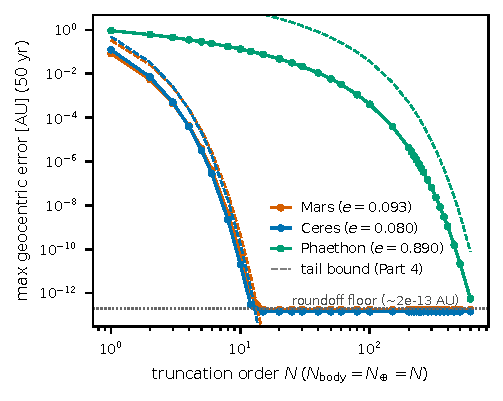
\includegraphics[width=\columnwidth]{fig_geo_convergence.pdf}
\caption{Maximum geocentric position error [AU] over a 50-yr window (daily
samples from JD 2461200.5) of the truncated epicycle chain with
$N_{\rm body}=N_\oplus=N$ versus exact Kepler motion, for Mars, Ceres and
Phaethon (solid), with the rigorous tail bound (dashed). Errors saturate at
the roundoff floor ($\sim2\times10^{-13}$~AU).}
\label{fig:conv}
\end{figure}

\subsection{Low-order truncations of Mars}
\label{sec:res-ptolemy}

Table~\ref{tab:ptolemy} gives the longitude error of truncations of the
geocentric Mars series in the planar approximation (coplanar J2000 mean
elements, $60$ yr at $0.5$~d steps, exact two-body reference, no light time or
aberration). The circular two-term approximation A, a single deferent and a single epicycle
($k=+1$ for both Mars and the Earth) with no eccentric offset and no equant,
reproduces all $28$ retrograde
loops of the true motion, which is the qualitative achievement of the epicycle
construction, but its longitude error reaches $33.2^\circ$ (RMS $9.7^\circ$), at perihelic
oppositions where the true distance is $0.37$~AU against $0.52$~AU in the
circular model. Adding the $k=0$ (eccentric) terms, model B, brings this to
$9.4^\circ$, and the equant-level model C to $5.05^\circ$. None of
these is a literal reproduction of Ptolemy's models, whose eccentric and equant
agree with the $k=0,1,2$ terms only to first order in $e$
\cite{Evans1984,Evans1988}; in particular model A is not Ptolemy's model, and
its $33.2^\circ$ error is not an assessment of Ptolemy's accuracy. The table says what a harmonic truncation of the
same order achieves. Truncation by retained set is not monotone at small
orders (E is slightly worse than D, because the retrograde terms shift errors
that partly cancelled), and a monotone decrease sets in only for
$|k|\le5$, where the error is $6\times10^{-4}$ degrees. The $N=5$ chain
($10+10$ rotating circles plus offsets) is within $0.001^\circ$ over the window of
Fig.~\ref{fig:retro}.

\begin{table}[H]
\caption{Low-order truncations of geocentric Mars (A is the circular two-term
approximation, with no eccentric and no equant), planar approximation,
$60$ years. Longitude error against the exact two-body motion; the true
number of retrograde intervals is $28$ and every model reproduces it.}
\label{tab:ptolemy}
\begin{ruledtabular}
\begin{tabular}{llrr}
Model & Retained terms & max ($^\circ$) & RMS ($^\circ$)\\
\hline
A & $k=1$, both bodies & $33.2$ & $9.7$\\
B & $k\in\{0,1\}$, both & $9.40$ & $2.7$\\
C & Mars $k\in\{0,1,2\}$, Earth $k=1$ & $5.05$ & $0.97$\\
D & $k\in\{0,1,2\}$, both & $0.557$ & $0.159$\\
E & $|k|\le2$, both & $0.728$ & $0.182$\\
F & $|k|\le5$, both & $6\times10^{-4}$ & $1\times10^{-4}$\\
G & $|k|\le10$, both & $<10^{-4}$ & $<10^{-4}$\\
\end{tabular}
\end{ruledtabular}
\end{table}

\begin{figure}[H]
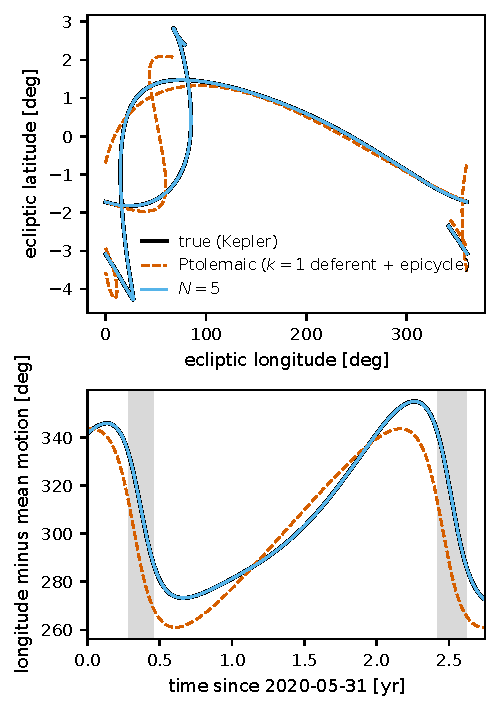
\includegraphics[width=\columnwidth]{fig_mars_retrograde.pdf}
\caption{Geocentric Mars over 2.75 years from 2020-05-31 (two oppositions).
Top: sky track in ecliptic longitude and latitude. Bottom: unwrapped longitude
minus its mean motion ($0.524^\circ$/day); grey bands mark retrograde motion
of the true path. Black: exact Kepler; dashed: circular two-term approximation
(Mars $k=+1$ deferent plus Earth $k=+1$ epicycle only, with no eccentric or
equant, so not Ptolemy's actual model; model A of
Table~\ref{tab:ptolemy}); blue: $N=5$ ($10+10$ rotating circles plus an offset each). The circular two-term approximation
reproduces the retrograde loops but is displaced by up to $32.8^\circ$ in
longitude in this window (planar 60-yr sup norm $33.2^\circ$, RMS
$9.7^\circ$); $N=5$ is within $0.001^\circ$.}
\label{fig:retro}
\end{figure}

\begin{figure}[H]
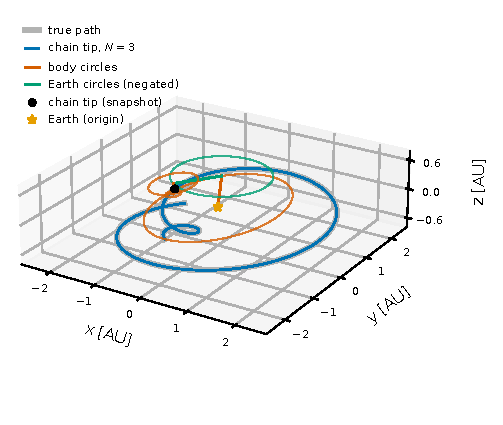
\includegraphics[width=\columnwidth]{fig_chain_3d.pdf}
\caption{Geocentric epicycle chain of Eros (inclination $10.8^\circ$) with
$N=3$ for Eros and for the Earth (12 rotating circles plus the static offsets, each circle drawn in its own orbital
plane about the preceding arm tip; red: body circles, green: negated Earth
circles). Blue: tip trail over one synodic period ($845$~d); grey: exact path.
Maximum tip error $0.01$~AU at this low order.}
\label{fig:chain3d}
\end{figure}

Figure~\ref{fig:chain3d} shows that inclination is handled without
modification: each circle lies in its own orbital plane, and the chain for
Eros ($i=10.8^\circ$) closes onto the exact path with the stated error.

\subsection{NAFF on Keplerian trajectories}
\label{sec:res-naff-kepler}

To validate the extraction we apply NAFF (Sec.~\ref{sec:num-naff}, Hann$^4$
window) to the \emph{exact} Keplerian geocentric Mars series over $200$ yr
sampled every $10$~d with $K=24$ lines, and match the lines to the analytic
Bessel terms. For the ten largest analytic terms the worst relative frequency
error is $2.0\times10^{-10}$ and the worst relative radius error is
$8.9\times10^{-8}$. On a $100$-yr Eros series ($5$-day sampling, $K=40$, $p=4$) the
reconstruction error is $7.6\times10^{-7}$~AU at worst over the full window
(record ends) and $3.1\times10^{-8}$~AU over the interior $80\%$. The data-driven extraction therefore rediscovers the analytic
epicycles; Table~\ref{tab:naff-lines} lists the ten circles with their
individual frequency, radius and phase errors.

\begin{table}[tb]
\caption{The ten largest analytic circles of the Keplerian geocentric Mars chain
($N_{\rm body}=N_\oplus=40$, excluding the static offset) and their recovery by NAFF
($200$ yr, $10$-day sampling, Hann$^4$ window, $K=24$). Circles, not lines:
the prograde and retrograde circles of one harmonic ($\pm k\,n_{\rm M}$) are
recovered from a single NAFF line and so share the same frequency error. $n_{\rm M}$ and
$n_\oplus$ are the mean motions of Mars and the Earth; the retrograde circles
$-k\,n_{\rm M}$ are those with negative index. Errors are relative for frequency and radius and
absolute (rad) for phase. Source: \texttt{experiments/out/naff\_lines\_mars.json}.}
\label{tab:naff-lines}
\begin{ruledtabular}
\footnotesize\setlength{\tabcolsep}{3pt}
\begin{tabular}{lrrrr}
Circle & Radius (AU) & $\delta\omega/\omega$ & $\delta r/r$ & $|\delta\phi|$\\
\hline
$+1 n_{\rm M}$ & 1.52 & $2.0\times10^{-10}$ & $8.9\times10^{-8}$ & $6.6\times10^{-8}$ \\
$+1 n_\oplus$ & 1.00 & $6.0\times10^{-11}$ & $6.5\times10^{-8}$ & $3.8\times10^{-8}$ \\
$+2 n_{\rm M}$ & $7.1\times10^{-2}$ & $2.1\times10^{-11}$ & $3.4\times10^{-8}$ & $1.4\times10^{-8}$ \\
$+2 n_\oplus$ & $8.4\times10^{-3}$ & $1.3\times10^{-11}$ & $1.6\times10^{-14}$ & $1.6\times10^{-8}$ \\
$+3 n_{\rm M}$ & $4.9\times10^{-3}$ & $7.2\times10^{-11}$ & $1.8\times10^{-13}$ & $7.2\times10^{-8}$ \\
$-1 n_{\rm M}$ & $1.7\times10^{-3}$ & $2.0\times10^{-10}$ & $8.9\times10^{-8}$ & $6.6\times10^{-8}$ \\
$+4 n_{\rm M}$ & $4.1\times10^{-4}$ & $1.2\times10^{-14}$ & $5.7\times10^{-13}$ & $7.5\times10^{-12}$ \\
$+3 n_\oplus$ & $1.0\times10^{-4}$ & $9.9\times10^{-11}$ & $2.6\times10^{-12}$ & $1.9\times10^{-7}$ \\
$-2 n_{\rm M}$ & $5.2\times10^{-5}$ & $2.1\times10^{-11}$ & $3.4\times10^{-8}$ & $1.4\times10^{-8}$ \\
$+5 n_{\rm M}$ & $3.7\times10^{-5}$ & $3.3\times10^{-11}$ & $2.0\times10^{-11}$ & $5.4\times10^{-8}$ \\
\end{tabular}
\end{ruledtabular}
\end{table}


\subsection{Perturbed Ceres}
\label{sec:res-ceres}

The Ceres test integrates the Sun, Earth, Jupiter, Saturn and a massless Ceres
over $200$ yr (5-day sampling, Sec.~\ref{sec:num-nbody}). A NAFF chain fitted
directly to the geocentric series would also have to absorb the
perturbations of the Earth, which a Kepler fit of Ceres alone cannot do, and the
NAFF window (Hann$^4$) weights the centre of the record much more strongly than
an unweighted least-squares fit does. To make the comparison like for like we
therefore fit the \emph{heliocentric} integrated Ceres trajectory in every case,
and subtract the \emph{same} integrated Earth trajectory from each reconstruction
before measuring the geocentric error, so that Earth-model error is excluded
from all rows. The Kepler baseline is a six-element least-squares fit, reported
both unweighted and weighted by the same Hann$^4$ window as NAFF (residual
weights $\sqrt w$). Errors are reported over the full window and over the interior
$80\%$ (Sec.~\ref{sec:num-baselines}).

Table~\ref{tab:ceres} gives the result. The interior error of the NAFF chain
decreases overall with the number of lines $K$, from $2.6\times10^{-2}$~AU at
$K=5$ to $1.7\times10^{-5}$~AU at $K=200$ (RMS $2.0\times10^{-6}$~AU). The
decrease is not monotone at the start: the interior maximum rises slightly from
$2.6\times10^{-2}$~AU at $K=5$ to $2.9\times10^{-2}$~AU at $K=10$ and decreases
monotonically for $K\ge10$, while the interior RMS decreases at every step. The NAFF interior maximum is
comparable to the fitted Kepler orbit ($2.7\times10^{-2}$~AU unweighted, RMS
$1.2\times10^{-2}$~AU) at $K=5$--$10$ and clearly smaller only for
$K\gtrsim50$ ($1.1\times10^{-2}$~AU at $K=50$, $1.1\times10^{-3}$~AU at
$K=100$). The full-window error does not fall: it lies between
$2.2\times10^{-2}$ and $4.4\times10^{-2}$~AU for all $K$ and grows with $K$ beyond
$K=20$, because the window vanishes at the record ends and the extra lines fit
the interior at the expense of the edges. The $K=200$ chain is therefore worse in
the maximum norm over the full window ($4.4\times10^{-2}$~AU) than either
Kepler fit ($3.7\times10^{-2}$~AU unweighted, $2.9\times10^{-2}$~AU weighted).
Weighting the Kepler fit by the Hann$^4$ window does not help it in the
interior: its interior maximum is slightly \emph{worse}
($2.8\times10^{-2}$ against $2.7\times10^{-2}$~AU) and only the full-window
maximum improves. Fitting NAFF to the geocentric series directly (the earlier
protocol, Fig.~\ref{fig:ceres}) gives interior errors larger by a factor of about $3$ at $K=200$ ($5.4\times10^{-5}$ against $1.7\times10^{-5}$~AU), and moving the Kepler baseline from the geocentric to the
heliocentric protocol changes its interior maximum only from
$2.74\times10^{-2}$ to $2.67\times10^{-2}$~AU. The comparison therefore does not
hinge on the Earth model, and we do not attribute the NAFF improvement to the
representation of Ceres alone: part of the difference between the two NAFF
protocols is the additional Earth lines that a geocentric fit must carry.
Osculating elements at the epoch give a much larger error, $0.89$~AU, an
artifact of osculating versus mean elements that we do not regard as a
meaningful comparison.

Figure~\ref{fig:ceresres} shows why the full-window and interior numbers
differ. The NAFF residuals are smallest at the centre of the record, rise
gradually towards both ends, and climb steeply within the first and last
$10\%$ to the size of the Kepler residuals, where the Hann$^4$ weight is
negligible and the fit is essentially unconstrained. This is the endpoint
effect, and it worsens as lines are added because they are placed to reduce the
weighted, mostly interior, residual. The Kepler residuals, weighted or not,
oscillate at the $10^{-2}$~AU level across the whole window, being limited by
the perturbation terms that a single ellipse cannot represent; the weighting
reshapes them only slightly.

\begin{table}[tb]
\caption{Perturbed Ceres, $200$ yr: maximum geocentric error [AU] of
reconstructions fitted to the \emph{heliocentric} integrated Ceres trajectory,
with the same integrated Earth subtracted from every row. NAFF with $K$ lines
($2K$ rotating circles plus a static offset), and six-element Kepler fits
unweighted and weighted by the Hann$^4$ window of NAFF.
$^a$Rotating circles, excluding the static offset.}
\label{tab:ceres}
\begin{ruledtabular}
\begin{tabular}{lrrr}
 & circles$^a$ & interior & full\\
\hline
NAFF $K=5$ & 10 & $2.6\times10^{-2}$ & $2.6\times10^{-2}$\\
NAFF $K=20$ & 40 & $1.9\times10^{-2}$ & $2.2\times10^{-2}$\\
NAFF $K=50$ & 100 & $1.1\times10^{-2}$ & $3.0\times10^{-2}$\\
NAFF $K=100$ & 200 & $1.1\times10^{-3}$ & $3.5\times10^{-2}$\\
NAFF $K=200$ & 400 & $1.7\times10^{-5}$ & $4.4\times10^{-2}$\\
Kepler fit, unweighted & 1 orbit & $2.7\times10^{-2}$ & $3.7\times10^{-2}$\\
Kepler fit, Hann$^4$-wtd & 1 orbit & $2.8\times10^{-2}$ & $2.9\times10^{-2}$\\
\end{tabular}
\end{ruledtabular}
\end{table}

\begin{figure}[H]
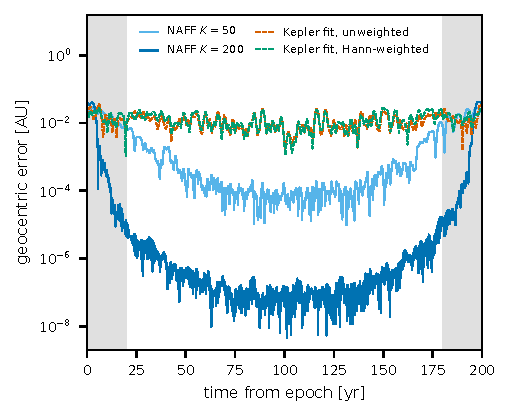
\includegraphics[width=\columnwidth]{fig_ceres_residual_time.pdf}
\caption{Geocentric position error [AU] of reconstructed Ceres versus time over the
$200$-yr N-body window, with the same integrated Earth subtracted from every
reconstruction. NAFF chains ($K=50$, $K=200$) are fitted to heliocentric Ceres
with the Hann$^4$ window; the six-element Kepler fits to heliocentric Ceres are
shown unweighted and weighted by the same window. Grey bands mark the first
and last $10\%$ of the record, outside the interior $80\%$ used for the interior
statistics. The NAFF errors rise towards the window ends, where the window
weight vanishes.}
\label{fig:ceresres}
\end{figure}

\begin{figure}[H]
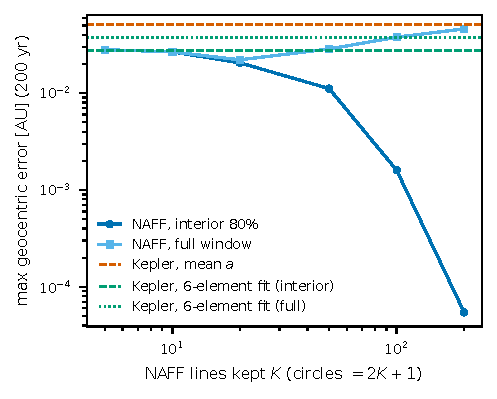
\includegraphics[width=\columnwidth]{fig_perturbed_ceres.pdf}
\caption{Maximum geocentric position error [AU] of a NAFF-extracted epicycle
chain ($2K$ rotating circles plus a static offset) fitted directly to the N-body (Sun, Earth, Jupiter, Saturn)
geocentric Ceres trajectory over 200 years (so Earth's perturbations are
fitted too), versus the number of lines $K$:
interior 80\% of the window (dark blue) and full window (light blue).
Horizontal lines: Kepler baselines that fit only Ceres with the Earth held on a Kepler orbit,
mean-$a$ Kepler $0.051$~AU and
6-element least-squares Kepler fit $0.027$~AU (interior), $0.038$~AU (full).
The osculating-element Kepler orbit (error $0.89$~AU) is omitted as an
element-offset artifact. The matched comparison is Table~\ref{tab:ceres}.}
\label{fig:ceres}
\end{figure}
